% !TEX root = main.tex
%%%%%%%%%%%%%%%%%%%%%%%%%%%%%%%%%%%%%%%%
%%%%%%%%%%%%%%%%%%%%%%%%%%%%%%%%%%%%%%%%
\section{\approach} \label{sec:t5}
%%%%%%%%%%%%%%%%%%%%%%%%%%%%%%%%%%%%%%%%
%%%%%%%%%%%%%%%%%%%%%%%%%%%%%%%%%%%%%%%%

We start by providing an introduction to the T5 model we use (\secref{sub:t5}). Then, we describe how we built the datasets used for the different training phases we deal with (\secref{sub:datasets}).  \secref{sec:training} will then explain how we used these datasets to run the actual training process.


\subsection{Text-to-Text-Transfer-Transformer (T5)}
\label{sub:t5}
T5 has been introduced by Raffel \etal \cite{raffel2019exploring} as a Transformer \cite{vaswani2017attention} model to support multitask learning. The idea behind T5 is to reframe NLP tasks in a unified text-to-text format in which the input and output of the model are text strings. The training of T5 includes two phases. The first is the \textit{pre-training}, in which the model is trained with a self-supervised objective to acquire general knowledge about the language(s) of interest. For example, this may mean providing as input to the model English sentences having a subset of their words masked and asking the model to generate as output the masked words. Being self-supervised (\ie the training instances can be automatically generated by masking random words) the pre-training can usually be performed on large-scale datasets. Once pre-trained, T5 can be fine-tuned to support specific tasks with supervised training objectives. This means, for example, providing it with pairs of sentences $<$\emph{english}, \emph{spanish}$>$ to train a translator.

In our work, we rely on the same T5 architecture (\ie T5$_{small}$) that has been exploited in LANCE \cite{mastropaolo2022using}. T5\textsubscript{\textit{small}} is characterized by six blocks for encoders and decoders. The feed-forward networks in each block consist of a dense layer with an output dimensionality ($d_{ff}$) of 2,048. The \textit{key} and \textit{value} matrices of all attention mechanisms have an inner dimensionality ($d_{kv}$) of 64, and all attention mechanisms have eight heads. All the other sub-layers and embeddings have a dimensionality ($d_{model}$) of 512. The code implementing T5 is available in our replication package \cite{replication}.


\subsection{Datasets Needed for Training, Validation, and Testing}
\label{sub:datasets}

We start by describing the dataset used for pre-training T5 (\secref{sub:pretraining}). Then, we detail the several fine-tuning datasets we built (featuring training, validation, and test set). The first, aimed at replicating LANCE \cite{mastropaolo2022using}, teaches T5 how to inject a single log statement in a \java method  (\secref{sec:single-log-dataset}). The second fine-tuning dataset also focuses on the problem of injecting a single log statement, but this time exploits IR to provide T5 with concrete examples of log messages that might be relevant for the prediction at hand (\secref{sec:single-log-plus-IR}). This allows to compare LANCE with \approach in the task of single log statement injection. The third fine-tuning dataset trains \approach for the task of multi-log statements prediction, \ie injecting from 1 to $n$ log statements in a given method (\secref{sec:multi-log-dataset}). Finally, we describe the fine-tuning dataset to train a T5 able to discriminate between methods \emph{needing} and \emph{not needing} log statements (\secref{sec:predicting-dataset}). The datasets are summarized in Tables \ref{tab:ds-summary-1} and \ref{tab:ds-summary-2} and available in \cite{replication}.


All datasets have been built starting from the same set of GitHub repositories that we selected using the GHS (GitHub Search) tool by Dabi\'c \etal \cite{dabic2021sampling}. GHS allows to query GitHub for projects meeting specific criteria. To this extent, we used the same selection criteria used in \cite{mastropaolo2022using}, selecting all public non-forked \java projects having at least 500 commits, 10 contributors, and 10 stars. These selection criteria aim at excluding personal/toy projects and reduce the chance of collecting duplicated code (non-forked repositories). We cloned the latest snapshot of the 6,352 projects returned by GHS. We scanned all cloned repositories to assess whether they featured a \texttt{POM} (Project Object Model) or a \texttt{build.gradle} file. Both these files allow to declare external dependencies towards libraries, the former using Maven, the latter Gradle. Such a check was performed since, as a subsequent step, we verify whether projects had a dependency towards Apache Log4j \cite{log4j} (\ie a well-known \java logging library) or SLF4J (Simple Logging Facade for \java) \cite{slf4j} (\ie an abstraction for \java logging frameworks similar to Log4j). Indeed, to train a T5 for the task of injecting complete log statement(s) in \java methods, we needed examples of methods featuring log statements. The usage of popular logging \java libraries was thus a prerequisite for the project's selection.

We found 3,865 projects having either a \texttt{POM} or a \texttt{build.gradle} file and 2,978 of them featured a dependency towards at least one logging library. The overall projects' selection is very similar to the one we performed in \cite{mastropaolo2022using}, with the main differences being the additional mining of projects: (i) using Gradle as build system (in \cite{mastropaolo2022using} only Maven was considered); and (ii) having a dependency towards SLF4J (in \cite{mastropaolo2022using} only Log4j was considered). These choices help in increase the size and variety of both the training and the testing datasets, making the prediction more challenging. 

We then used srcML \cite{srcml} to extracted all \java methods in the selected projects. Then, we identified the log statements within each method (if any) and removed all methods featuring log statements exploiting custom log levels (\ie log levels that do not belong to any of the two libraries we consider, but that have been defined within a specific project). The valid log levels we considered are: \texttt{FATAL}, \texttt{ERROR}, \texttt{WARN}, \texttt{DEBUG}, \texttt{INFO}, and \texttt{TRACE}. At this point we were left with two sets of methods: those not having any log statement and those having at least one log statement using one of the ``valid'' log levels.

We run \emph{javalang} \cite{javalang} on the remaining methods to tokenize them and excluded all those having $\#tokens < 10$ or $\#tokens \geq 512$. The upper-bound filtering has been done in previous works \cite{mastropaolo2021empirical,tufano2021automating,ciniselli2021empirical,tufano-mutants,Tufano:tosem2019} to limit the computational expenses of training DL-based models. 

The lower-bound of 10 tokens aims at removing empty methods. We also removed all methods containing non-ASCII characters in an attempt to exclude at least some of the methods featuring log messages not written in English. Finally, to avoid any possible overlap between the training, evaluation, and test datasets we are going to create from the collected set of methods, we removed all exact duplicates, obtaining the final set of 12,916,063 \java methods, of which 244,588 contain at least one log statement. 

\begin{table*}[h]
	\centering
	\scriptsize
	\caption{Number of methods in the datasets used in our study\vspace{-0.3cm}}
		\label{tab:ds-summary-1}
	\begin{tabular}{ccccccccc}
		\toprule
		\multirow{2}{*}{\textit{\textbf{Dataset}}} & \multicolumn{2}{c}{\textbf{train}} & \textbf{} & \textbf{eval} & \textbf{} & \textbf{test}  \\ \cline{2-3} \cline{5-5} \cline{7-7} 
		& \textbf{w/ log} & \textbf{w/o log} & \textbf{} & \textbf{w/ log} & \textbf{} & \textbf{w/ log} \\ \midrule
		\textit{Pre-training}              & -               &      12,671,475  &           & -               &           &  -               \\
		\textit{Fine-tuning: Single Log Generation}               & 229,703         & -                &           & 28,763          &           & 28,698          \\
		\textit{Fine-tuning: Single Log Generation with IR}               & 229,703         & -                &           & 28,763          &           & 28,698          \\
		\textit{Fine-tuning: Multi-log Injection with IR}               & 192,773         & -                &           & 24,092         &           & 24,088          \\
		\bottomrule
	\end{tabular}
	\vspace{-0.3cm}
\end{table*}

\subsubsection{Pre-Training Dataset}
\label{sub:pretraining}
Since the goal of pre-training is to provide T5 with general knowledge about the language of interest (\ie \java), we used for pre-training all methods not featuring a log statement (the latter will be used for the fine-tuning datasets). We adopted a classic \emph{masked language model} task, which consists in randomly masking 15\% of the tokens composing a training instance (\ie a \java method) asking the model to predict them. 


\figref{fig:pre-training} depicts the masking procedure of instances used to pre-train the model.


\begin{figure}[h!]
	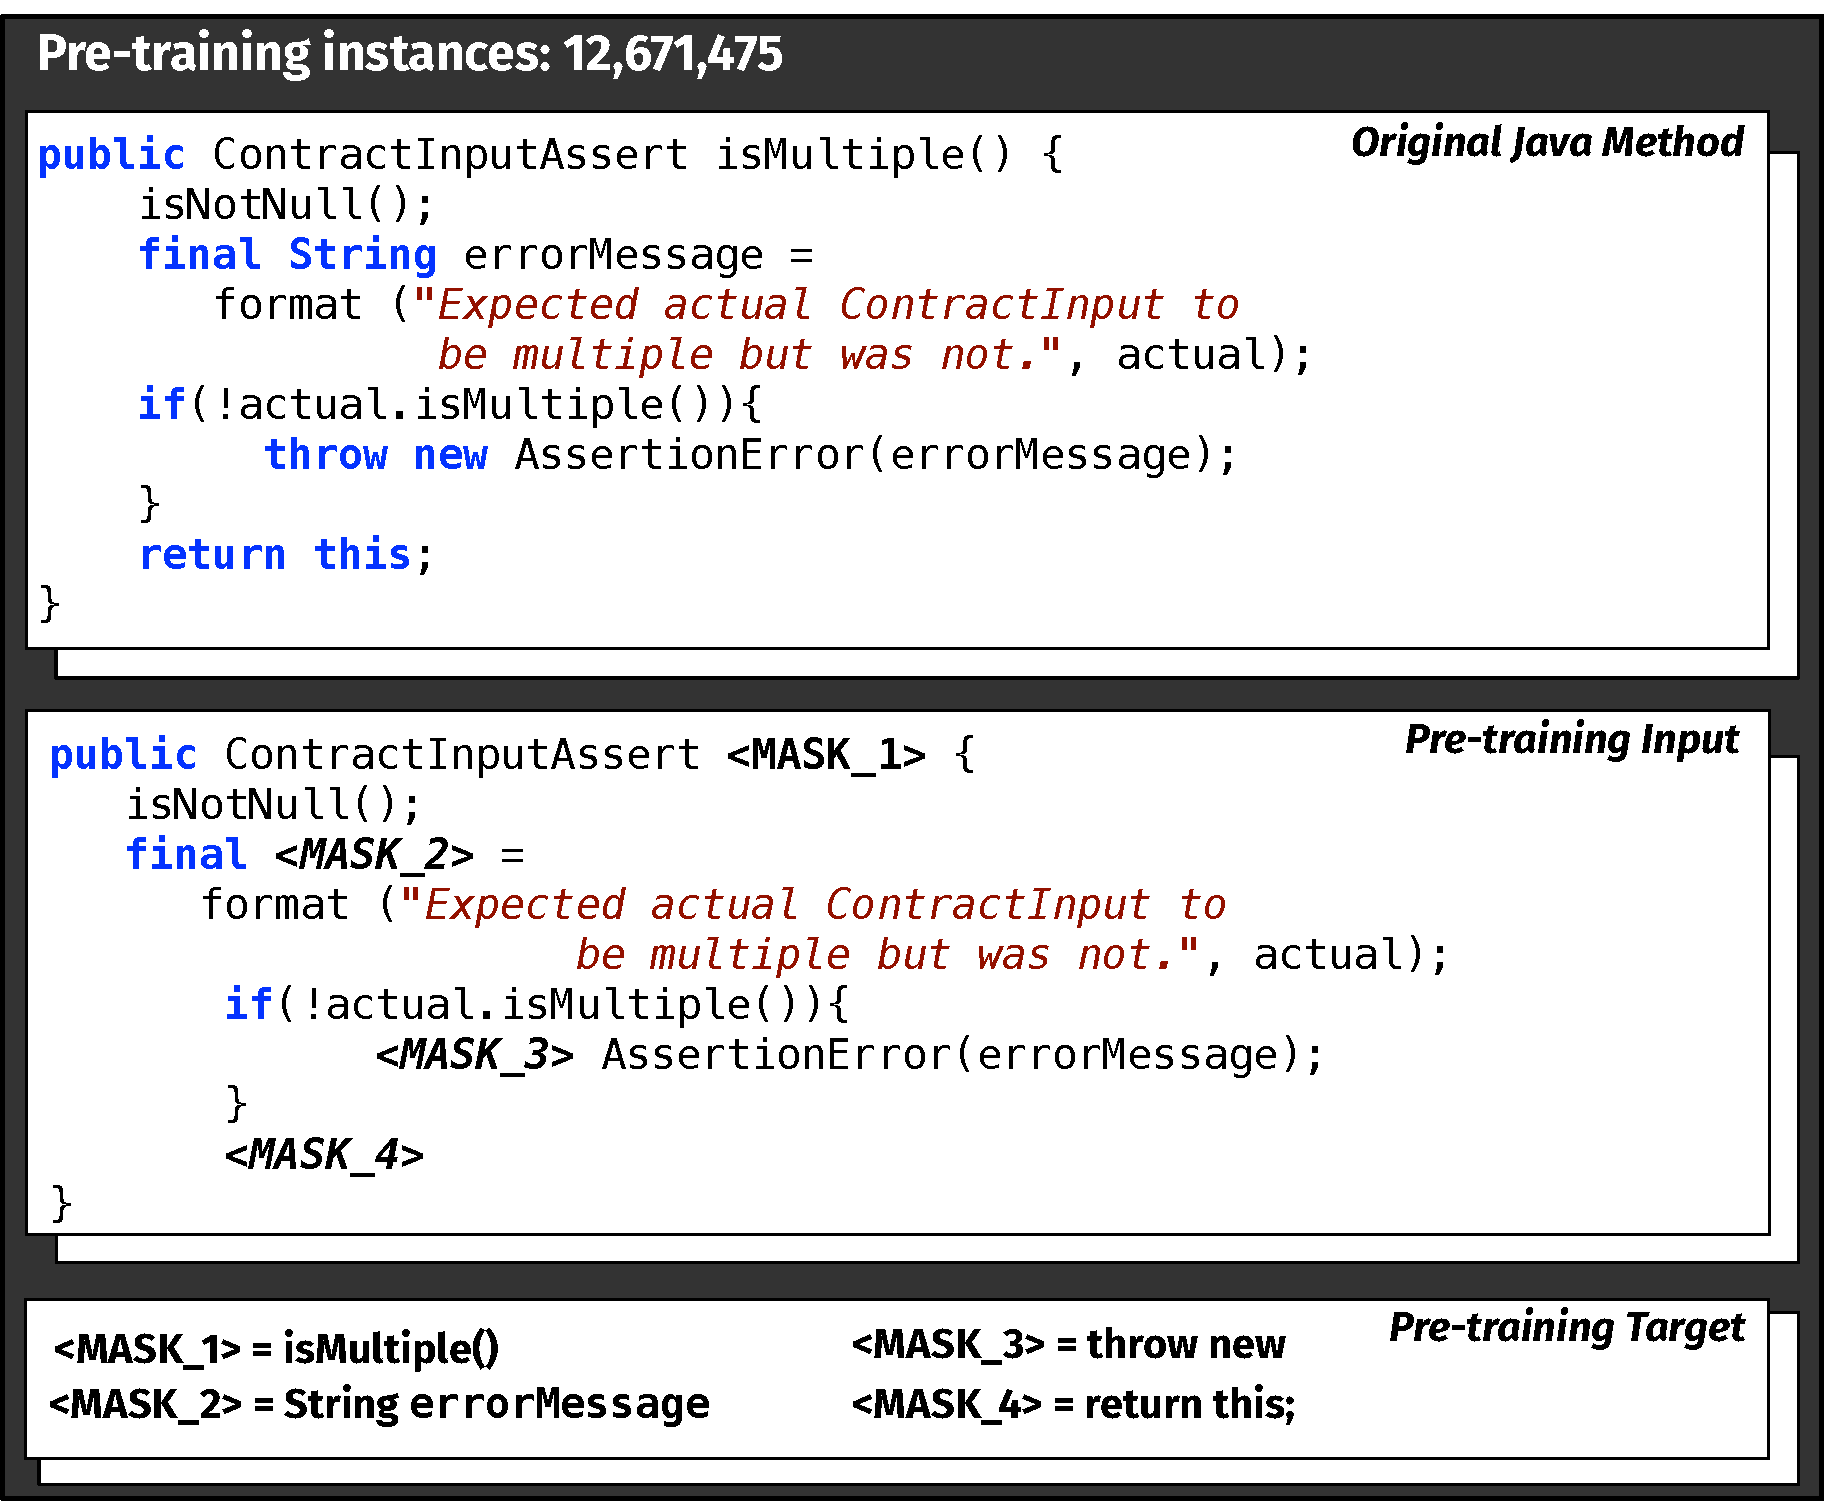
\includegraphics[width=0.70\columnwidth]{img/pre-training.pdf}
	\caption{Example of Pre-training instance}
	\label{fig:pre-training}
\end{figure}



\subsubsection{Fine-tuning Dataset: Single Log Generation} \label{sec:single-log-dataset}
We build a fine-tuning aimed at replicating what has been done in the training of LANCE \cite{mastropaolo2022using}. We process each method $M$ having $n \geq 1$ log statements by removing from it one log statement (\ie leaving it with $n-1$ log statements). This allows to create a training pair $\langle M_s, M_t \rangle$ with $M_s$ representing the input provided to the model (\ie $M$ with one removed log statement) and  $M_t$ being the expected output (\ie $M$ in its original form, with all its log statements). This is the dataset used to train LANCE \cite{mastropaolo2022using} and it allows to train a model able, given a \java method as input, to inject in it one new log statement. For methods having $n > 1$ (\ie more than one log statement), we created $n$ pairs $\langle M_s, M_t \rangle$, each of them having one of the $n$ log statements removed (\ie different $M_s$). To ensure that after the log statement removal our instances still featured valid \java methods, we parsed each $M_s$ using JavaParser \cite{javaparser} and removed all pairs including an invalid $M_s$. 

We split the remaining pairs into training (80\%), validation (10\%) and test (10\%) set as reported in \tabref{tab:ds-summary-1}. Training and testing a T5 model on this dataset basically means performing a differentiated replication of LANCE on a 3.6$\times$ larger and more variegate (multiple logging libraries) dataset.

\subsubsection{Fine-tuning Dataset: Single Log Generation with IR} \label{sec:single-log-plus-IR}

In \approach, we combine DL and IR with the goal of boosting performance especially in the generation of meaningful log messages. The main idea is to augment the input provided to the model (\ie $M_{s}$) with log messages belonging methods similar to $M_{s}$ which are featured in the training set. For each of the 244,588 $\langle M_s, M_t \rangle$ pairs in the fine-tuning dataset described in \secref{sec:single-log-dataset} (this includes training, validation, and test), we identify the $k$ most similar pairs in the training set. The similarity between two pairs is based on the similarity of their $M_s$ (\ie the method in which the log statement must be created) and it is computed using the Jaccard similarity \cite{hancock2004jaccard} index, based on the percentage of code tokens shared across the two methods. We then use these $k$ similar methods to extract from them examples of log messages used in coding contexts which are similar to the $M_s$ at hand. 

Two clarifications are needed. First, independently if a given pair is in the training, validation, or test set, we extract its $k$ most similar pairs only from the training set. This is needed since, while predicting the log statement to inject, the training set must be the only knowledge available to the model (\ie the test set must be composed of previously unseen instances). Second, when computing the Jaccard similarity, we remove from the compared methods all log statements, since we want to identify similar ``coding contexts'' that may require similar log statements. We created three different fine-tuning datasets using different values of $k=\{1,3,5\}$ (thus, a higher/lower number of exemplar log messages provided to the model).

\begin{figure}[h!]
	\centering
	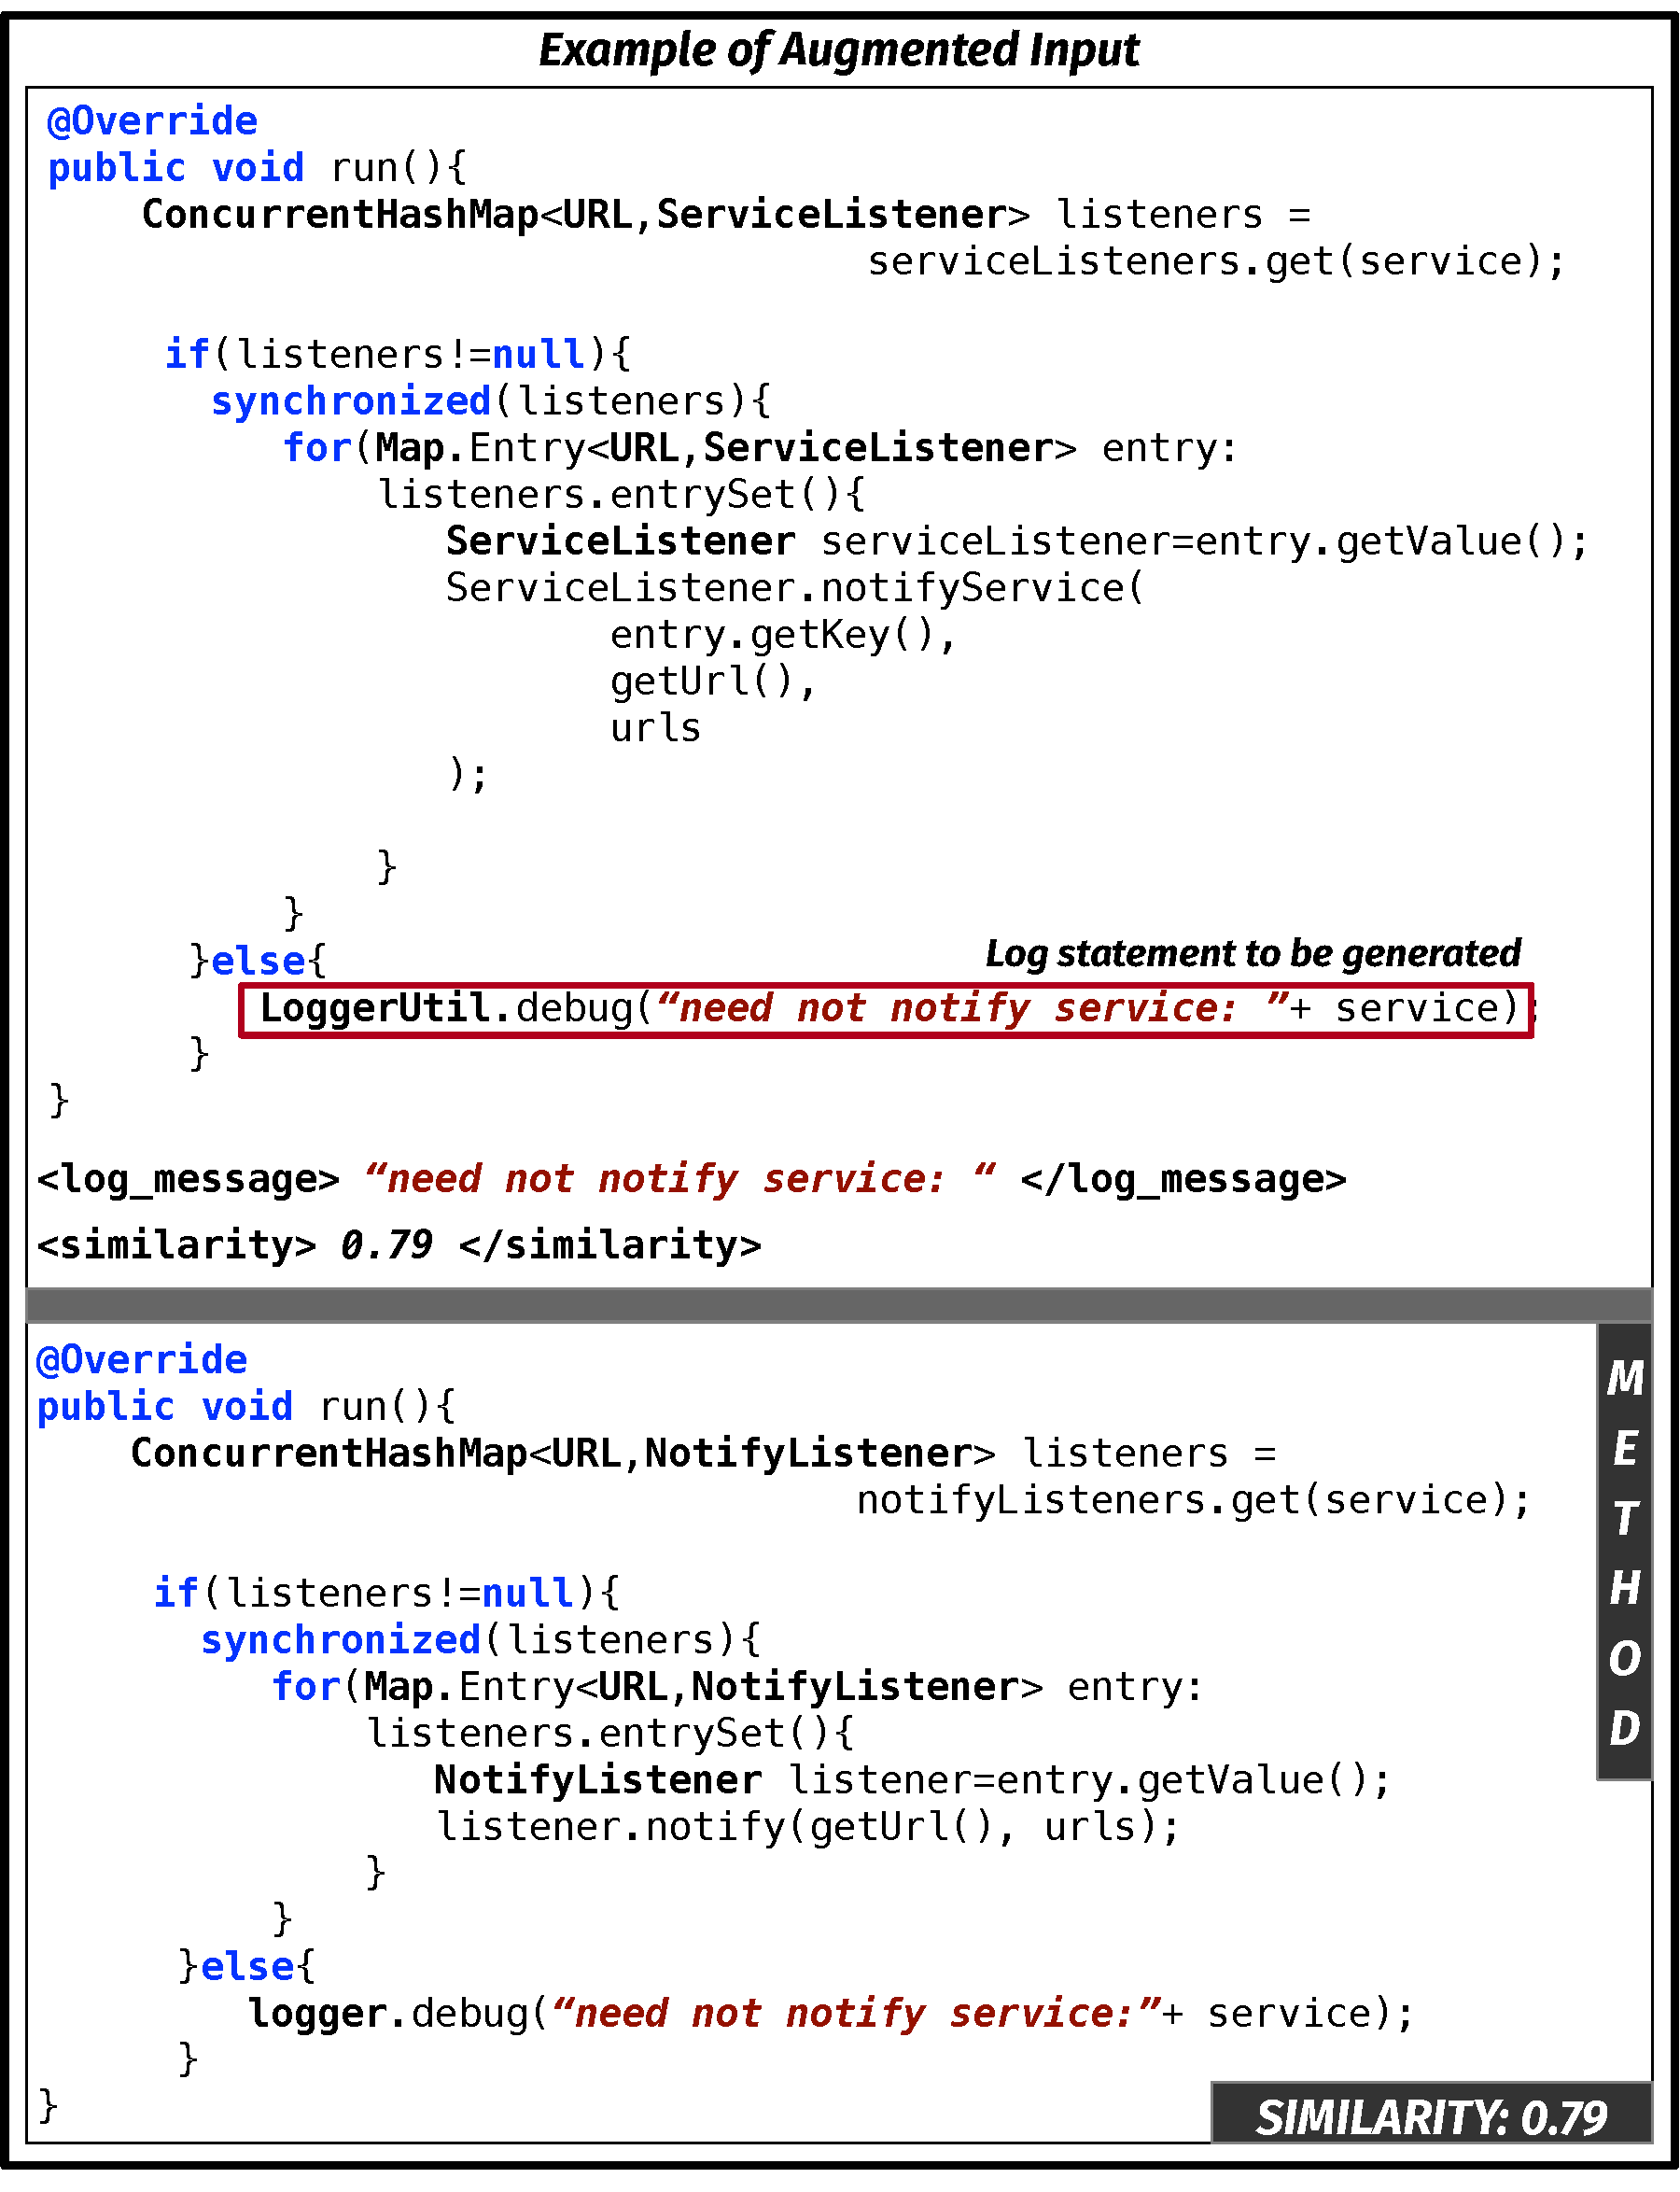
\includegraphics[width=0.70\columnwidth]{img/ir-example.pdf}
	\vspace{-0.2cm}
	\caption{Example of instance in the ``Single Log Generation with IR'' dataset}
	\label{fig:ir-example}
\end{figure}


\figref{fig:ir-example} shows an example of training instance for this fine-tuning dataset. The method on top represents the $M_{s}$ \java method in which a log statement must be injected (\ie the one highlighted in red). The method is enriched with the exemplar log messages that have been found in the $k=1$ most similar method shown in the bottom. Besides the log messages, we also provide T5 with the Jaccard similarity between the $M_{s}$ at hand (top of the figure in this case) and the method of the training set from which the exemplar log message(s) has been extracted. 

This is meant to provide T5 with an additional hint in terms of which exemplar message comes from the most similar coding context (when more messages are retrieved).

Note that the instances in this dataset are exactly the same of the one previously described to replicate LANCE (see \tabref{tab:ds-summary-1}). This allows a direct comparison in terms of performance which will provide information about the gain, if any, provided by the IR integration.


\subsubsection{Fine-tuning Dataset: Multi-log Injection with IR} \label{sec:multi-log-dataset}

One limitation of LANCE \cite{mastropaolo2022using} we aim at addressing in this extension, is the assumption that a \java method provided as input always requires one new log statement to be injected. Also for this dataset, \approach exploits a combination of DL and IR, thus we follow a process similar to the one described in \secref{sec:single-log-plus-IR}, with the main difference being the number of log statements we ask the model to generate. Given a method $M$ featuring $n$ log statements, we randomly select $y$ log statements to remove from it, with $1 \leq y \leq n$. This means that we create pairs $\langle M_s, M_t \rangle$ in which $M_s$ lacks a ``random'' number of log statements that must be generated by the model to obtain the target method $M_t$. This makes the prediction task substantially more challenging as compared to the single-log injection scenario experimented in LANCE. Also in this case we parsed each $M_s$ using JavaParser \cite{javaparser} and removed all pairs including an invalid $M_s$. The remaining part of the process (\ie identifying the $k$ most similar pairs to inject examples of log messages) is the same described in \secref{sec:single-log-plus-IR}. \tabref{tab:ds-summary-1} shows the distribution of instances among the training, evaluation, and test set for this dataset as well.


\subsubsection{Fine-tuning Dataset: Deciding Whether Log Statements are Needed} \label{sec:predicting-dataset}

While the dataset described in \secref{sec:multi-log-dataset} allows to build a model able to inject multiple log statements in a given \java method, such a model still assumes that at least one log statement must be injected in the input method. Thus, \approach also includes a T5 model trained as a binary classifier in charge of deciding whether a method provided as input requires the addition of log statements or not. In case of affirmative answer, the method can then be passed to the previously trained model which will decide how many and which log statements to inject.

\begin{table*}[h!]
	\centering
	\scriptsize
	\caption{Number of methods in the datasets used to predict the need for log statements\vspace{-0.3cm}}
	\begin{tabular}{rcccccccc}
		\toprule
		\multirow{2}{*}{\textit{\textbf{Dataset}}} & \multicolumn{2}{c}{\textbf{train}} & \textbf{} & \multicolumn{2}{c}{\textbf{eval}}  & \textbf{} & \multicolumn{2}{c}{\textbf{test}}  \\ \cline{2-3} \cline{5-6} \cline{8-9} 
		& \textbf{Need} & \textbf{No need}   & \textbf{} & \textbf{Need} & \textbf{No need}   & \textbf{} & \textbf{Need} & \textbf{No need}   \\ \midrule
		\textit{Fine-tuning: Need4Log (50-50)}         & 98,848        & 92,126             &           & 12,257        & 11,468             &           & 11,627        &  11,627            \\
		\textit{Fine-tuning: Need4Log (75-25)}         & 98,848        & 92,126             &           & 12,257        & 11,468             &           & 12,159        &  4,053             \\
		\textit{Fine-tuning: Need4Log (25-75)}         & 98,848        & 92,126             &           & 12,257        & 11,468             &           & 3,875         &  11,627            \\ 
		\textit{Fine-tuning: Need4Log (2-98)}         & 98,848        & 92,126             &           & 12,257        & 11,468             &           & 238         &  11,627            \\ 
		\bottomrule
	\end{tabular}
	\label{tab:ds-summary-2}
\end{table*}

To train such a classifier we again start from the original set of 244,588 \java methods having at least one log statement. Then, similarly to what done in \secref{sec:multi-log-dataset}, given a method $M$ featuring $n$ log statements, we randomly select $y$ log statements to remove from it with, however, $0 \leq y \leq n$. Thus, differently from the training dataset used for multi-log injection, we have instances from which we did not remove any log statement ($y=0$). 

Then, we create a pair $\langle M_s, B \rangle$ in which $M_s$ is the original method $M$ \textbf{possibly} lacking a random number of log statements, while $B$ is a boolean variable that could be equal \emph{true} (\ie $M_s$ needs the addition of log statements, since $y \geq 1$) or \emph{false} (\ie no log statements are needed in $M_s$, since $y = 0$). Non-parsable methods resulting after the removal of the log statements have then been removed, as well as duplicates resulting from different methods that, after the removal of log statements, become equal (\ie their only differences were the removed log statements). This process resulted in a dataset featuring 190,974 training instances (98,848 needing at least a log statement and 92,126 not needing it), accompanied by the evaluation and test sets summarized in \tabref{tab:ds-summary-2}.

As it can be seen, four different versions of the test set have been created, to experiment \approach in different scenarios. Let us explain such a choice. The test set should be representative of the real distribution of methods \emph{needing} and \emph{not needing} log statements. However, such a distribution cannot be computed in a reliable way. Indeed, one possibility we considered to build our dataset was to just consider all methods with and without log statements as training instances (as opposed to work only with methods having at least a log statement as we do). In a nutshell, the process would have been: (i) remove a random number of log statements from the methods with at least one log statement to create instances \emph{needing} logs; and (ii) assume that all methods without log statements do not require logging. However, assuming that all methods in a project not having log statements do not require logging is a very strong assumption. It is indeed possible that the project's developers just did not consider yet the usage of logs in a specific method or that, in a given project, logging is not yet a practice at all (thus all methods do not use log statements). This makes difficult a reliable computation of the number of methods \emph{needing} and \emph{not needing} logging. Also, such a problem justifies our decision to create instances of methods \emph{needing}/\emph{not needing} a log statement starting from all methods having at least one log statement and using the process described above (\ie removing a random number of statements to create instances in need of logging, and not removing any log statement to create instances not needing logging). At least, we are sure that these are methods for which developers considered logging (since they have at least one log statement) and, thus, can be seen as a sort of ``oracle''. 

The four test sets in \tabref{tab:ds-summary-2} simulate four different distributions of methods \emph{needing}/\emph{not needing} log statements: balanced (50\% per category), unbalanced towards \emph{needing} (75\%-25\%), unbalanced towards \emph{not needing} (25\%-75\%), and strongly unbalanced towards \emph{not needing} (2\%-98\%). 

The latter is a distribution we computed based on all 12M+ methods we mined, in which 98\% of methods do not have log statements, while 2\% have it. As said, this distribution is not completely reliable but, at least, gives an idea of what we found in the mined projects.



\section{Training and Hyperparameter Tuning} \label{sec:training}
All training we performed have been run using a Google Colab's 2x2, 8 cores TPU topology with a batch size of 128.

\subsection{Tokenizer Training}
Since we use software-specific corpora for pre-training and fine-tuning, we trained a tokenizer (\ie a SentencePiece model \cite{kudo2018sentencepiece}) on 1M \java methods (randomly extracted from the pre-training dataset) and 712,634 English sentences from the C4 dataset \cite{raffel2019exploring}. We included English sentences since, once fine-tuned, the models may be required to synthesize with complex (natural language) log messages. We set the size of the vocabulary to 32k word-pieces.

\subsection{Pre-training}
We pre-trained T5 for 500k steps on the pre-training dataset composed by 12,671,475 \java methods (\tabref{tab:ds-summary-1}). Given the size of our dataset and the batch size, 500k steps correspond to $\sim$5 epochs. The maximum size of the input/output was set to 512 tokens.

\begin{table*}[h!]
	\centering
	\caption{T5 hyperparameter tuning results (in bold the best learning rate)\vspace{-0.3cm}}
	\begin{tabular}{lrrrr}
		\toprule
		\textbf{Experiment}                  																		& \textbf{C-LR}              & \textbf{ST-LR}      & \textbf{ISQ-LR}        & \textbf{PD-LR} \\
		\midrule
		\textit{Fine-tuning: Single Log Generation with IR} ($k=1$)                         &   24.63\%                & 25.92\%    		           & \textbf{26.55\%}           &  26.36\%         \\
		\textit{Fine-tuning: Single Log Generation with IR} ($k=3$)                        &   26.25\%                & 26.04\%    		           & \textbf{26.68\%}          &  26.33\%         \\
		\textit{Fine-tuning: Single Log Generation with IR} ($k=5$)                         &  26.24\%                & 25.69\%    		           & \textbf{26.78\%}           &  26.33\%         \\
		\midrule
		\textit{Fine-tuning: Multi-log Generation with IR} ($k=1$)                         &   22.62\%                & 22.19\%    		           & \textbf{22.79\%}           &  22.76\%         \\
		\textit{Fine-tuning: Multi-log Generation with IR} ($k=3$)                        &   22.64\%                & 22.28\%    		           & \textbf{23.05\%}          &  22.59\%         \\
		\textit{Fine-tuning: Multi-log Generation with IR} ($k=5$)                         &   22.71\%                & 22.14\%    		           & \textbf{22.78\%}           &  22.51\%         \\
		\midrule
		\textit{Fine-tuning: Need4Log} & 96.58\%       & 96.56\%        & 96.59\%          & \textbf{96.62\%}\\
		\bottomrule
	\end{tabular}
	\vspace{-0.3cm}
	\label{tab:hp-results}
\end{table*}

\subsection{Hyperparameter Tuning}
Once pre-trained the model, we finetune the hyperparameters of the model following the same procedure we employed when developing LANCE. Such a procedure has been executed for each of the fine-tuning datasets previously described. In particular, we assessed the performance of T5 when using four different learning rate scheduler: (i) \textit{Constant Learning Rate} (C-LR): the learning rate is fixed during the whole training; (ii) \textit{Inverse Square Root Learning Rate} (ISR-LR): the learning rate decays as the inverse square root of the training step; (iii) \textit{Slanted Triangular Learning Rate \cite{howard2018universal}} (ST-LR): the learning rate first linearly increases and then linearly decays to the starting learning rate; and (iv) \textit{Polynomial Decay Learning Rate} (PD-LR): the learning rate decays polynomially from an initial value to an ending value in the given decay steps. 
The exact configuration of all the parameters used for each scheduling strategy is reported in \tabref{tab:learning-rates}.


\begin{table}[h]
	\centering
	\caption{Configurations for the experimented learning rates}
	\begin{tabular}{ll}
		\hline
		\textbf{Learning Rate Type} & \textbf{Parameters}               \\ \hline
		Constant                     & \textit{LR = 0.001}               \\
		Inverse Square Root         & \textit{LR\textsubscript{starting} = 0.01}  \\
		& \textit{Warmup = 10,000}          \\
		Slanted Triangular          & \textit{LR\textsubscript{starting} = 0.001} \\
		& \textit{LR\textsubscript{max} = 0.01}       \\
		& \textit{Ratio = 32}               \\
		& \textit{Cut = 0.1}                \\
		Polynomial Decay            & \textit{LR\textsubscript{starting} = 0.01}  \\
		& \textit{LR\textsubscript{end} = 0.001}      \\
		& \textit{Power = 0.5}              \\ \hline
	\end{tabular}
	\label{tab:learning-rates}
\end{table}

Each model has been run for 100k training steps on the fine-tuning dataset. Then, its performance has been assessed on the evaluation set in terms of correct predictions (\ie cases in which the generated output is equal to the target one). 

For the generative models injecting log statements this means that they outputted the \java method featuring all correct log statements in the expected positions. For the classifier, it means that it correctly predicted the need for log statements in a given method. The results achieved with each learning rate are reported in \tabref{tab:hp-results}. Our hyperparameter tuning required training and evaluating 28 models: For each of the 7 fine-tuning datasets in \tabref{tab:hp-results} we experimented 4 different learning rates. Given the achieved results, we will use the ISQ-LR for the generative models, and the PD-LR for the classifier when fine-tuning the models. Concerning the ``replication of LANCE'' (\ie fine-tuning T5 on the dataset \emph{Fine-tuning: Single Log Generation} in \tabref{tab:ds-summary-1}), we did not perform any hyperparameter tuning, but relied on the best configuration reported in the original paper \cite{mastropaolo2021studying}, thus using the PD-LR.



\subsection{Fine-tuning}
Once identified the best learning rates to use, we fine-tuned the final models using early stopping, with checkpoints saved every 10k steps, a delta of 0.01, and a patience of 5. This means training the model on the fine-tuning dataset and evaluating its performance (again in terms of correct predictions) on the evaluation set every 10k. The training process stops if a gain lower than delta (0.01) is observed at each  50k steps interval. This means that after 60k steps, the performance of the model is compared against that of the 10k checkpoint and, if the gain in performance is lower than 0.01, the training stops and the best-performing checkpoint up to that training step is selected. This process has been used for all models, including the one replicating LANCE. Our replication package \cite{replication} reports the convergence of all models (\ie the steps after which the early stopping criterion was met). 


\subsection{Generating Predictions}
Once the T5 models have been pre-trained and fine-tuned, they can be used to generate predictions for the targeted tasks. We generate predictions using a greedy decoding strategy, meaning that the generated prediction is the result of selecting at each decoding step the token with the highest probability of appearing in a specific position. Thus, a single prediction (\ie the one maximizing the likelihood of among all the produced tokens) is generated for an input sequence, as compared to strategies such as beam-search \cite{freitag2017beam} that generate multiple predictions.
